\message{ !name(main.tex)}\documentclass{beamer}
\usepackage[utf8]{inputenc}
 
\usepackage[square,numbers]{natbib}
\usepackage{graphicx}
\usepackage{amsmath,amsfonts,amssymb,amsthm}
\usepackage{thmtools}
\usepackage{stmaryrd}
\usepackage{url}
\usepackage{array}
\usepackage{arydshln}
\usepackage{ifthen}
\usepackage{ifpdf}
\usepackage{verbatim}
\usepackage{listings}
\usepackage{mathpartir}

\usepackage{mathtools}
\DeclarePairedDelimiter\ceil{\lceil}{\rceil}
\DeclarePairedDelimiter\floor{\lfloor}{\rfloor}

\usepackage{appendix}

\usepackage{tikz}
\usepackage{multirow}

\newcommand{\forcenewline}{$\phantom{v}$\\}
\newcommand{\judgment}[2]{\paragraph{#1}\hspace{\stretch{1}}\fbox{$#2$}}

\newcommand{\update}[2]{[#1 \mapsto #2]}
\newcommand{\sem}[1]{\left\llbracket #1 \right\rrbracket}

%Math notation
\newcommand{\restrictfun}[1]{|_{#1}}
\newcommand{\parfun}{\rightharpoonup}
\newcommand{\finparfun}{\xrightharpoonup{\textit{\tiny{fin}}}}
\newcommand{\monnefun}{\xrightarrow{\textit{\tiny{mon, ne}}}}
\newcommand{\monfun}{\xrightarrow{\textit{\tiny{mon}}}}
\newcommand{\nefun}{\xrightarrow{\textit{\tiny{ne}}}}
\newcommand{\fun}{\rightarrow}
\newcommand{\defeq}{\stackrel{\textit{\tiny{def}}}{=}}
\newcommand{\nequal}[1][n]{\stackrel{\tiny{#1}}{=}}
\newcommand{\nsubeq}[1][n]{\stackrel{\tiny{#1}}{\subseteq}}
\newcommand{\nsupeq}[1][n]{\stackrel{\tiny{#1}}{\supseteq}}
\newcommand{\union}{\mathbin{\cup}}
\DeclareMathOperator{\dom}{dom}
\newcommand{\blater}{\mathop{\blacktriangleright}}
\newcommand{\id}{\var{id}}
\newcommand{\undefined}{\mathit{undefined}}

\newcommand{\powerset}[1]{\mathcal{P}(#1)}

\newcommand{\false}{\mathit{false}}
\newcommand{\true}{\mathit{true}}

%cofes
\newcommand{\cofe}{c.o.f.e.}
\newcommand{\cofes}{\cofe{}'s}
\newcommand{\CatC}{\mathbb{C}}
\newcommand{\CatP}{\mathbb{P}}

%Comments
\newcommand\lau[1]{{\color{purple} \sf \footnotesize {LS: #1}}\\}
\newcommand\dominique[1]{{\color{purple} \sf \footnotesize {DD: #1}}\\}
\newcommand\lars[1]{{\color{purple} \sf \footnotesize {LB: #1}}\\}

%Variables
\newcommand{\var}[1]{\mathit{#1}}
\newcommand{\hs}{\var{hs}}
\newcommand{\hv}{\var{hv}}
\newcommand{\rv}{\var{rv}}
\newcommand{\lv}{\var{lv}}
\newcommand{\gl}{\var{g}}
\newcommand{\pc}{\mathit{pc}}
\newcommand{\pcreg}{\mathrm{pc}}
\newcommand{\addr}{\var{a}}
\newcommand{\offset}{\var{offset}}
\newcommand{\word}{\var{w}}
\newcommand{\start}{\var{base}}
\newcommand{\addrend}{\var{end}}
\newcommand{\pwlv}{\var{pwl}}
\newcommand{\mem}{\var{mem}}
\newcommand{\reg}{\var{reg}}
\newcommand{\heapseg}{\var{hs}}
\newcommand{\heap}{\var{heap}}
\newcommand{\perm}{\var{perm}}
\newcommand{\permp}{\var{permPair}}
\newcommand{\roll}{\var{roll}}
\newcommand{\instr}{\var{instr}}
\newcommand{\stdcap}[1][\perm]{\left(#1,\start,\addrend,\addr \right)}

%Memory projections
\newcommand{\plainproj}[1]{\mathrm{#1}}
\newcommand{\memheap}[1][\Phi]{#1.\plainproj{heap}}
\newcommand{\memreg}[1][\Phi]{#1.\plainproj{reg}}

\newcommand{\updateHeap}[3][\Phi]{#1\update{\plainproj{heap}.#2}{#3}}
\newcommand{\updateReg}[3][\Phi]{#1\update{\plainproj{reg}.#2}{#3}}

%Configuration end states
\newcommand{\failed}{\textsl{failed}}
\newcommand{\halted}{\textsl{halted}}

%Functions
\newcommand{\plainfun}[2]{
  \ifthenelse{\equal{#2}{}}
             {\mathit{#1}}
             {\mathit{#1}(#2)}
}
\newcommand{\decode}{\plainfun{decode}{}}
\newcommand{\encode}{\plainfun{encode}{}}
\newcommand{\encodePerm}{\plainfun{encodePerm}{}}
\newcommand{\decodePerm}{\plainfun{decodePerm}{}}
\newcommand{\updatePcPerm}[1]{\plainfun{updatePcPerm}{#1}}

\newcommand{\executeAllowed}[1]{\plainfun{executeAllowed}{#1}}
\newcommand{\nonZero}[1]{\plainfun{nonZero}{#1}}
\newcommand{\readAllowed}[1]{\plainfun{readAllowed}{#1}}
\newcommand{\writeAllowed}[1]{\plainfun{writeAllowed}{#1}}
\newcommand{\withinBounds}[1]{\plainfun{withinBounds}{#1}}
\newcommand{\stdUpdatePc}[1]{\plainfun{updatePc}{#1}}

\newcommand{\readCond}[1]{\plainfun{readCondition}{#1}}
\newcommand{\writeCond}[1]{\plainfun{writeCondition}{#1}}
\newcommand{\execCond}[1]{\plainfun{executeCondition}{#1}}
\newcommand{\entryCond}[1]{\plainfun{entryCondition}{#1}}

\newcommand{\revokeTemp}[1]{\plainfun{revokeTemp}{#1}}
\newcommand{\erase}[2]{\floor*{#1}_{\{#2\}}}


%World operations
\newcommand{\future}{\mathbin{\sqsupseteq}}
\newcommand{\futurewk}{\mathbin{\sqsupseteq}_{\var{wk}}}
\newcommand{\futurestr}{\mathbin{\sqsupseteq}_{\var{str}}}
\newcommand{\heapSat}[3][\heap]{#1 :_{#2} #3}

\newcommand{\monwknefun}{\xrightarrow[\text{\tiny{$\futurewk$}}]{\textit{\tiny{mon, ne}}}}
\newcommand{\monstrnefun}{\xrightarrow[\text{\tiny{$\futurestr$}}]{\textit{\tiny{mon, ne}}}}


%Assembly labels
\newcommand{\codelabel}[1]{\mathit{#1}}
\newcommand{\init}{\codelabel{init}}
\newcommand{\malloc}{\codelabel{malloc}}
\newcommand{\counter}{\codelabel{counter}}
\newcommand{\iocap}{\codelabel{iocap}}

%Type(s)
\newcommand{\type}[1]{\mathrm{#1}}
\newcommand{\asmType}{\plaindom{AsmType}}


%Domains
\newcommand{\plaindom}[1]{\mathrm{#1}}
\newcommand{\Caps}{\plaindom{Cap}}
\newcommand{\Words}{\plaindom{Word}}
\newcommand{\Addrs}{\plaindom{Addr}}
\newcommand{\Mems}{\plaindom{Mem}}
\newcommand{\RegName}{\plaindom{RegisterName}}
\newcommand{\Regs}{\plaindom{Reg}}
\newcommand{\Heaps}{\plaindom{Heap}}
\newcommand{\HeapSegments}{\plaindom{HeapSegment}}
\newcommand{\Confs}{\plaindom{Conf}}
\newcommand{\Instrs}{\plaindom{Instructions}}
\newcommand{\nats}{\mathbb{N}}
\newcommand{\ints}{\mathbb{Z}}
\newcommand{\Perms}{\plaindom{Perm}}
\newcommand{\Globals}{\plaindom{Global}}

\newcommand{\Rel}{\plaindom{Rel}}
\newcommand{\States}{\plaindom{State}}
\newcommand{\RegionNames}{\plaindom{RegionName}}
\newcommand{\Regions}{\plaindom{Region}}
\newcommand{\Reg}{\plaindom{Reg}}
\newcommand{\Worlds}{\plaindom{World}}
\newcommand{\Wor}{\plaindom{Wor}}
\newcommand{\Worwk}{\Wor_{\futurewk}}
\newcommand{\Worstr}{\Wor_{\futurestr}}
\newcommand{\xiwk}{\xi_{\var{wk}}}
\newcommand{\xistr}{\xi_{\var{str}}}
\newcommand{\StorePred}{\plaindom{HeapSegPred}}
\newcommand{\UPred}[1]{\plaindom{UPred}(#1)}
\newcommand{\DCPred}[1]{\plaindom{P}^\downarrow(#1)}

\newcommand{\Views}{\plaindom{View}}

%LR
\newcommand{\intr}[2]{\mathcal{#1}}
\newcommand{\valueintr}[1]{\intr{V}{#1}}
\newcommand{\exprintr}[1]{\intr{E}{#1}}
\newcommand{\contintr}[1]{\intr{K}{#1}}
\newcommand{\regintr}[1]{\intr{R}{#1}}
\newcommand{\stdvr}{\valueintr{\asmType}}
\newcommand{\stder}{\exprintr{\asmType}}
\newcommand{\stdrr}{\regintr{\asmType}}
\newcommand{\stdkr}{\contintr{\asmType}}
\newcommand{\observations}{\mathcal{O}}
\newcommand{\npair}[2][n]{\left(#1,#2 \right)}

%Reference register/heap
\newcommand{\refreg}[1]{\lfloor #1 \rfloor}
\newcommand{\refheap}[1]{\langle #1 \rangle_h}

%Instructions
%No arguments
\newcommand{\zinstr}[1]{\mathtt{#1}}
\newcommand{\fail}{\zinstr{fail}}
\newcommand{\halt}{\zinstr{halt}}
%One argument
\newcommand{\oneinstr}[2]{\zinstr{#1} \; #2}
\newcommand{\jmp}[1]{\oneinstr{jmp}{#1}}
%Two arguments
\newcommand{\twoinstr}[3]{\zinstr{#1} \; #2 \; #3}
\newcommand{\jnz}[2]{\twoinstr{jnz}{#1}{#2}}
\newcommand{\isptr}[2]{\twoinstr{isptr}{#1}{#2}}
\newcommand{\setptr}[2]{\twoinstr{setptr}{#1}{#2}}
\newcommand{\move}[2]{\twoinstr{move}{#1}{#2}}
\newcommand{\store}[2]{\twoinstr{store}{#1}{#2}}
\newcommand{\load}[2]{\twoinstr{load}{#1}{#2}}
\newcommand{\lea}[2]{\twoinstr{lea}{#1}{#2}}
%Three arguments
\newcommand{\threeinstr}[4]{\zinstr{#1} \; #2 \; #3 \; #4}
\newcommand{\restrict}[3]{\threeinstr{restrict}{#1}{#2}{#3}}
\newcommand{\subseg}[3]{\threeinstr{subseg}{#1}{#2}{#3}}
\newcommand{\plus}[3]{\threeinstr{plus}{#1}{#2}{#3}}

%Permissions
\newcommand{\plainperm}[1]{\mathrm{#1}}
\newcommand{\noperm}{\plainperm{o}}
\newcommand{\readonly}{\plainperm{ro}}
\newcommand{\readwrite}{\plainperm{rw}}
\newcommand{\exec}{\plainperm{rx}}
\newcommand{\entry}{\plainperm{e}}
\newcommand{\rwx}{\plainperm{rwx}}
%PWL permissions
\newcommand{\readwritel}{\plainperm{rwl}}
\newcommand{\rwlx}{\plainperm{rwlx}}

%Global/local
\newcommand{\local}{\plainperm{local}}
\newcommand{\glob}{\plainperm{global}}

\newcommand{\localReg}{\var{localReg}}
\newcommand{\globalReg}{\var{globalReg}}

%Views
\newcommand{\plainview}[1]{\mathrm{#1}}
\newcommand{\perma}{\plainview{perm}}
\newcommand{\temp}{\plainview{temp}}
\newcommand{\revoked}{\plainview{revoked}}

%OP sem
\newcommand{\diverge}[1][n]{\not\Downarrow_{#1}}
\newcommand{\step}[1][]{\rightarrow_{#1}}

\newsavebox{\locstatebox}
\newsavebox{\tdbox}

\title{Reasoning about capability machines using logical relations}
\author{Lau Skorstengaard}
\institute{Aarhus University}
\date{KU Leuven, November 2016}
\begin{document}

\message{ !name(main.tex) !offset(-3) }

\frame{\titlepage}

\frame{
  \frametitle{Capabilities}
  What is a capability? \pause
  \begin{itemize}
  \item<2-> \emph{Unforgeable} token of authority
    %What this means depends on system
  \end{itemize} \pause
  What is a capability in a capability machine?
  \begin{itemize}
  \item<4-> Unforgeable pointer
    % In a normal machine, you can use an integer as a pointer (not unforgeable)
    % No way to generate capabilities.
    % System enforces this.
  \item<5-> Range of memory
    % Authority over range of memory, may be one cell, doesn't have to be.
  \item<6-> Permission
    % Kind of authority.
    % What can this capability be used for.
  \end{itemize}
  \begin{onlyenv}<4-6>
  \begin{figure}
    \centering
    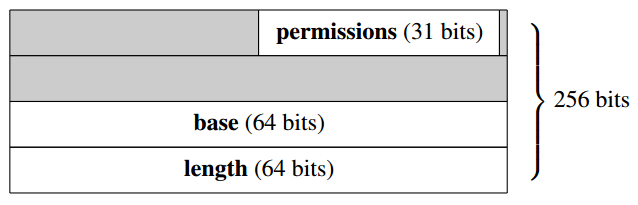
\includegraphics[width=0.8\textwidth]{chericap}
    \caption{CHERI capability \cite{Woodruff:2014:CCM:2665671.2665740}}
    \label{fig:chericap}
  \end{figure}
\end{onlyenv}
}

\frame{
\frametitle{Capability Permissions}
\begin{itemize}
\item Read
\item Write
\item Execute
\item<2-> Enter
  \begin{itemize}
  \item<3-> When jumped to, it becomes and execute capability. 
  \end{itemize}
\end{itemize}
}

\frame{
\frametitle{Capability Machine Instructions}
\begin{itemize}
\item<1-> Same instructions as in a normal low-level machine
  \begin{itemize}
  \item<2-> \texttt{\emph<3>{jmp}}, \texttt{\emph<3>{jnz}}, \texttt{move}, \texttt{plus}, \texttt{\emph<3>{load}}, \texttt{\emph<3>{store}}
  \item<3-> Instructions may require capability with certain permission.
    %jmp has to be to an execute capability
    %load has to be through a read capability
    %store has to be through a write capability
  \end{itemize}
\item<4-> Capability manipulation instructions
  \begin{itemize}
  \item<5-> \texttt{lea}, \texttt{restrict}, \texttt{subseg} 
  \item<6-> No instruction generates new capability
  \item<7-> Manipulation of capabilities cannot result in authority amplification
  \end{itemize}
\end{itemize}
}

\frame{
\frametitle{Capability Machine Overview}
\begin{itemize}[<+->]
\item Capabilities 
  \begin{itemize}
  \item Permissions
  \item Range of authority
  \end{itemize}
\item Capability aware instructions
\item Heap and registers
  \begin{itemize}
  \item Can contain data and capabilities
    %Capabilities can be distinguished from data using tagging (file or bit in cap).
  \end{itemize}
\end{itemize}
}

\frame{
\frametitle{Formalisation}
\begin{itemize}[<+->]
\item A mathematical model of the system
\item Allows us to reason formally about the system
\item May make some abstractions
\item Needs to stay true to the original system
\end{itemize}
}

\frame{
  \frametitle{Formalisation - Permissions}
  \textbf{Permissions}
  \begin{itemize}
  \item To simplify matters, we only allow certain combinations of permissions
  \item<2-> No permisions, \onslide<3->{read only,} \onslide<4->{read-write,} \onslide<5->{read-execute,} \onslide<6->{entry,} \onslide<7->{read-write-execute}
  \end{itemize}

  \[
    \Perms \defeq \{ \onslide<2->{\noperm,} \onslide<3->{\readonly,} \onslide<4->{\readwrite,} \onslide<5->{\exec,} \onslide<6->{\entry,} \onslide<7->{\rwx}\}
  \]
}

\frame{
  \frametitle{Formalisation - Capabilities}

  \textbf{Capability}
  \begin{itemize}
  \item<2-> Permission
  \item<4-> Range og authority
  \item<7-> Pointer
  \end{itemize}

  \[
    \onslide<5->{\Addrs \defeq \nats}
  \]

  \[
    \Caps \defeq \onslide<3->{\Perms} \onslide<6->{\times \Addrs \times \Addrs} \onslide<8->{\times \Addrs}
  \]
  \onslide<9->{
    Example: $(\entry, 30, 42, 30)$
  }
}

\frame{
  \frametitle{Formalisation - Words and register file}
  \textbf{Words}
  \begin{itemize}
  \item<2-> Capability
  \item<4-> Data (and instructions)
  \end{itemize}
  \[
    \Words \defeq \onslide<3->{\Caps} \onslide<5->{+ \ints}
  \]
  \onslide<6->{
    \textbf{Register file}
    \begin{itemize}
    \item<7-> Assume finite set of registers $\RegName$ with $\pcreg$
    \end{itemize}
    \[
      \Regs \defeq \onslide<8->{\RegName \rightarrow \Words}
    \]
  }
}

\frame{
  \frametitle{Formalisation - Heap and configurations}
  \textbf{Heap}
  \begin{itemize}
  \item \emph{Total} map from $\Addrs$ to $\Words$
  \end{itemize}
  \[
    \Heaps \defeq \Addrs \rightarrow \Words 
  \]

  \textbf{Configuration}
  \begin{itemize}
  \item Executable configuration
  \item Successfully halted configuration
  \item Failed configuration
  \end{itemize}
  \[
    \Confs \defeq \Regs \times \Heaps + \{ \failed \} + \{\halted\} \times \Mems
  \]
}

\begin{frame}
  \frametitle{Formalisation - Instructions}
  \textbf{Syntax}
  \begin{itemize}
  \item The normal instructions
  \item The capability manipulation instructions
  \item Instructions for stopping the machine
  \end{itemize}
  $$\begin{array}{rcl}
   \Instrs &::=& \jmp{\lv} \mid \jnz{\lv}{\rv} \mid \move{\lv}{\rv} \mid \\
           &   & \load{\lv}{\hv} \mid \store{\hv}{\rv} \mid \plus{\lv}{\rv}{\rv} \mid\\
           &   & \lea{\lv}{\rv} \mid \restrict{\lv}{\rv}{\rv} \mid  \\
           &   & \subseg{\lv}{\rv}{\rv} \mid \fail \mid \halt

  \end{array}$$

\end{frame}

\begin{frame}
  \frametitle{Formalisation - Operational Semantics (1)}
  \[
    \step \subseteq (\Regs \times \Heaps) \times \Confs
  \]

  \begin{mathpar}
    \inferrule{ \memreg(\pcreg) = \stdcap \\ 
                \start \leq \addr < \addrend \\
                \perm \in \{ \exec,\rwx\} }
              { \var{executionAllowed}(\Phi) }
    \and
    \inferrule{ \var{executionAllowed}(\Phi) }
              { \Phi \step \sem{\decode(\memheap(\addr))}(\Phi) }
    \and
    \inferrule{ \neg \var{executionAllowed}(\Phi) }
              { \Phi \step \failed }
  \end{mathpar}
\end{frame}

\begin{frame}
  \frametitle{Formalisation - Operational Semantics (2)}
    \begin{mathpar}
      \inferrule{ \memreg(\pcreg) = \stdcap \\
        \var{newPc} = (\perm,\start,\addrend,\addr + 1)}
      { \stdUpdatePc{\Phi} = \updateReg{\pcreg}{\var{newPc}} }

      \onslide<2>{\and  
      \inferrule{\memreg(r_2) = \stdcap\\
        \perm \in \{\readonly, \readwrite, \exec, \rwx \} \\
        \start \leq \addr \leq \addrend \\
        \var{w} = \memheap(\addr)}
      {\sem{\load{\refreg{r_1}}{\refheap{r_2}}}(\Phi) = \stdUpdatePc{\updateReg{r_1}{\var{w}}}}}
    \onslide<3>{\and
      \inferrule{ \memreg(\rv_1) = \stdcap \\
        \rv_2 = n \lor \memreg(\rv_2) = n\\
        n \in \ints\\
        \var{newPerm} = \decodePerm(n)\\
        \var{newPerm} \sqsubseteq \perm\\
        c = (\var{newPerm},\start,\addrend,\addr) }
      { \sem{\restrict{\refreg{r_1}}{\rv_1}{\rv_2}} = \stdUpdatePc{\updateReg{r_1}{\var{c}}} }}
    \end{mathpar}
\end{frame}

\begin{frame}[fragile]
  \frametitle{Program examples}
  \begin{itemize}
  \item High-level programs
  \item \texttt{let x = 0 in ...} - allocates a new cell on the heap and sets the value to 0.
  \item \texttt{assert(l == 1)} - if the assertion is true, then execution continues. If the assertion is false, then some designated heap cell is set to 1 and execution halts.
  \end{itemize}

  \begin{block}{}
\begin{verbatim}
let f = fun adv =>
          let l = 1 in
          adv();
          assert (l == 1)
\end{verbatim}
\begin{block}{Lemma}
  Given any program \texttt{adv}, \texttt{f(adv)} either runs forever, ends up in the \failed{} configuration, or halts in 
\end{block}

\end{block}


\begin{block}{}
\begin{verbatim}
fun adv =>
  let c = 0 in
  let td = (fun _ =>
              c := !c + 1) in
  adv(td);
  assert(c >= 0)
\end{verbatim}
\end{block}
\end{frame}

\frame{
\frametitle{Logical Relation}

}

\frame{
\frametitle{Example programs revisited}

}

\frame{
\frametitle{Local capabilities}
}

\frame{
  \bibliographystyle{plainnat}
  \bibliography{refs}
}

\end{document}
\message{ !name(main.tex) !offset(-552) }
